\chapter{"Квазипланковский" спектр капиллярной турбулентности на поверхности жидкого водорода}

Несмотря на то, что теория турбулентных каскадов существует не одно десятилетие и построено немало моделей волновой турбулентности, а также производились многочисленные вычислительные эксперименты, до сих пор не было произведено экспериментального исследования диссипативной области турбулентного каскада. Такие эксперименты требуют достаточного уровня развития компьютерной техники для оцифровки аналоговых сигналов и последующей их обработки. Тем не менее эти эксперименты необходимы, поскольку диссипация энергии является важной составляющей турбулентного каскада и понимание процессов диссипации необходимо для исследования вопроса накопления и перераспределения энергии в турбулентном каскаде. %\todo{расставить ссылки}

В этой главе представлено исследование диссипативной области турбулентного каскада в системе капиллярных волн на поверхности жидкого водорода. При изучении волновой турбулентности жидкий водород выгодно отличается от воды в четыре раза более низким коэффициентом кинематической вязкости и в три раза большим коэффициентом нелинейности капиллярных волн. Таким образом относительная ширина инерционного интервала (определенная как отношение характерных частот диссипации энергии $\omega_b$ к частоте накачке $\omega_p$) оценивается из соотношения нелинейности и вязкого затухания капиллярных волн. Оценка показывает, что относительная ширина инерционного интервала для жидкого водорода в три раза больше, чем для воды.\todo{расставить ссылки на формулы}

\section{Экспериментальная методика} %\label{sect1_1}
 Экспериментальная установка состоит из оптической ячейки расположенной в вакуумной полости гелиевого криостата и оптической системы регистрации колебаний на поверхности жидкости. Проводящий цилиндрический сосуд 6 мм глубиной и 60 мм диаметром был установлен внутри ячейки, а проводящая пластина зафиксирована в 4 мм над сосудом. Газообразный водород сконденсирован в сосуде. Радиоактивная мишень(молибденовая пластина, покрытая слоем тритида титана), расположенная в нижней части сосуда, ионизирует жидкий водород. В присутствии постоянного напряжения около 1 кВ между сосудом и верхней пластиной, ионы разделяются и заряды со знаком соответствующим полярности постоянного напряжения собираются под поверхностью жидкого водорода. Волны на поверхности жидкого водорода возбуждаются добавочное переменное напряжение с максимальной амплитудой 100 В. Более подробно эта методика возбуждения волн описана в \cite{Brazhnikov_IET}

\begin{figure}[ht] 
  \center
  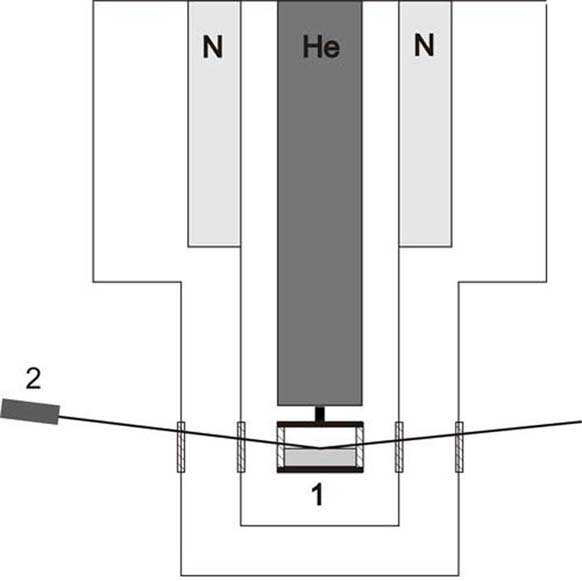
\includegraphics [scale=0.4] {article1/kriostat.jpg}
  \caption{Схематичная конструкция криостата.
  1 – экспериментальная ячейка, 2 – лазер.} 
%  \label{img:hydr_specrta_dlog}  
\end{figure}


\begin{figure}[ht] 
  \center
  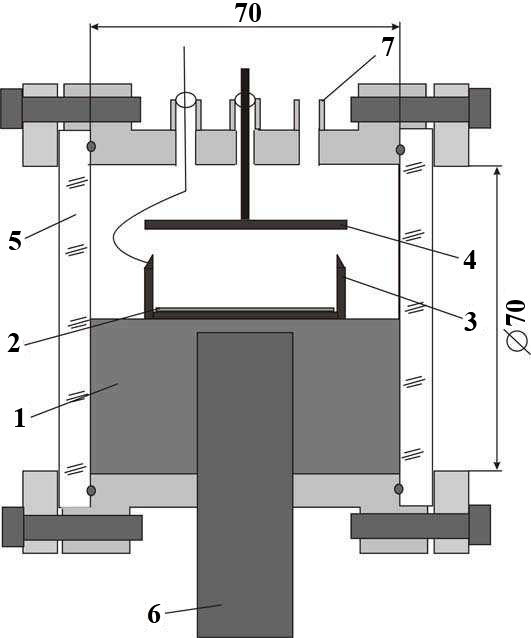
\includegraphics [scale=0.4] {article1/cell.jpg}
  \caption{Схематичная конструкция ячейки. 
  1 – текстолитовый брусок, 2 – радиоактивная мишень, 3 – медный контейнер, 4 – верхняя обкладка конденсатора, 5 – кварцевое окно, 6 - медный хладопровод, 7 – капилляр для набора водорода.} 
%  \label{img:hydr_specrta_dlog}  
\end{figure}


	Использование электрического поля для создания капиллярных волн дает большое преимущество по сравнению с использованием техник возбуждения волн на поверхности воды, например неустойчивость Фарадея. Это позволяет нам возбуждать поверхность аккуратно достаточно хорошо контролируемой силой. В этой серии экспериментов в качестве переменного возбуждающего напряжения были использованы низкочастотные случайные сигналы. Эти сигналы были синтезированы через Фурье-преобразование случайного набора фаз и прямоугольного амплитудного спектра, которые везде равен нулю кроме заданного частотного интервала(интервал накачки).
	
\begin{figure}[ht] 
  \center
  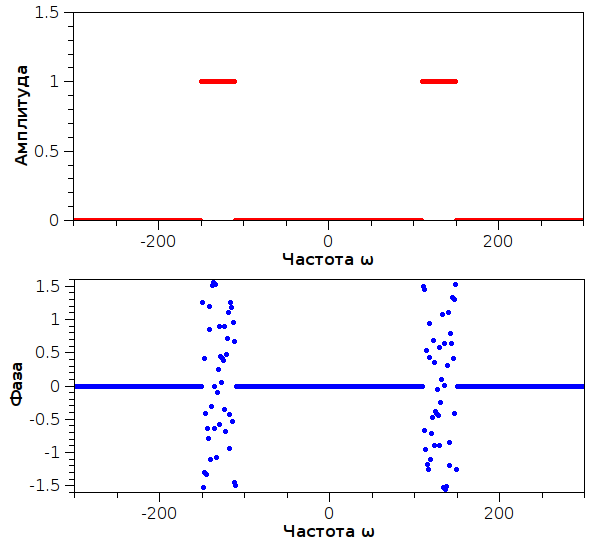
\includegraphics [scale=0.75] {article1/ftt-gen1.png}
  \caption{Частотное распределение амплитуды (верхний график) и пример частотного распределения фазы (нижний рисунок) сигнала, использующегося в качестве накачки.} 
%  \label{img:hydr_specrta_dlog}  
\end{figure}
\begin{figure}[ht] 
  \center
  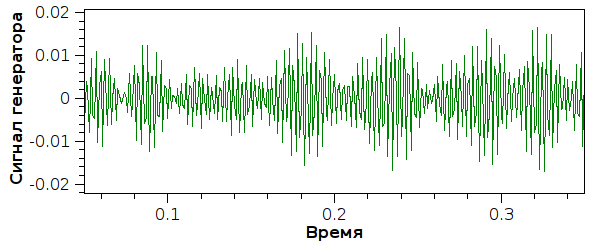
\includegraphics [scale=0.75] {article1/fft-gen2.png}
  \caption{Фрагмент сигнала накачки.} 
%  \label{img:hydr_specrta_dlog}  
\end{figure}


	Для регистрации волн на поверхности жидкости использовался метод отражения лазерного луча. Лазерный луч падает под малым скользящим лучом(около 0.2 рад) на поверхность жидкости, отражается и фокусируется линзой на фотодетектор. Напряжение на фотодетекторе усиливается и оцифровывается 24 битным аналогоцифровым преобразователем с частотой дискретизации около 100 кГц. Волны регистрировались в режиме "широкого луча", когда размер лазерного луча больше, чем характерная длина волны. Энергия отраженного лазерного луча $P(t)$  в этом режиме пропорциональна отклонению поверхности $\eta(t)$ \cite{Brazhnikov_bound_freq}. По этой причине в дальнейшем не делается разницы между спектром корреляционной функции отклонения поверхности $<|\eta_\omega^2|>$ и энергии отраженного лазерного луча $<P_\omega^2>$. Более подробно эта методика измерения описана в \cite{Brazhnikov_IET}.

	Максимальная крутизна волны которая может быть зарегистрирована в эксперименте ограничена размером оптических окон криостата и приблизительно равно 0.05 рад.

\section{Экспериментальные результаты и обсуждение} %\label{sect1_1}
 Капиллярные волны возбуждались случайной силой в частотном диапазоне 39-103 Гц. Средний квадрат возбуждающего напряжения менялся от $V_p = 0$ В, т.е. отсутствие накачки, до $V_p = 30$ В, ограничение связано с максимальной крутизной волны. На рис. \ref{img:hydr_specrta_dlog} показан пример Фурье-спектра для отраженной энергии лазерного луча $P_\omega^2$ для разных амплитуд возбуждающей силы. На рис \ref{img:hydr_specrta_dlog} хорошо видно область накачки на низкочастотной части спектра. За областью накачки следует инерционный интервал - относительно широкая частотная область, где видна степенная зависимость спектра $P_\omega^2$. Ширина инерционного интервала зависит от амплитуды накачки. Когда поверхность возбуждается слабо (переменное напряжение $V_p = 4$ В) диссипация начинается рядом с областью накачки и инерционный интервал не наблюдается. Увеличение силы накачки приводит к уширению инерционного интервала, высокочастотная граница инерционного интервала $\omega_b$ смещается к высоким частотам. Наиболее широкий инерционный интервал с границами от $\approx 0.3$ кГц, до $\omega_b \approx 4$ кГц наблюдается при максимальном напряжении накачки $V_p = 30$ В. На частотах выше высокочастотной границы колебания поверхности затухают из-за вязких потерь, кривая $P_\omega^2$ идет вниз гладко и уходит ниже уровень аппаратных шумов.
 
 \begin{figure}[ht] 
  \center
  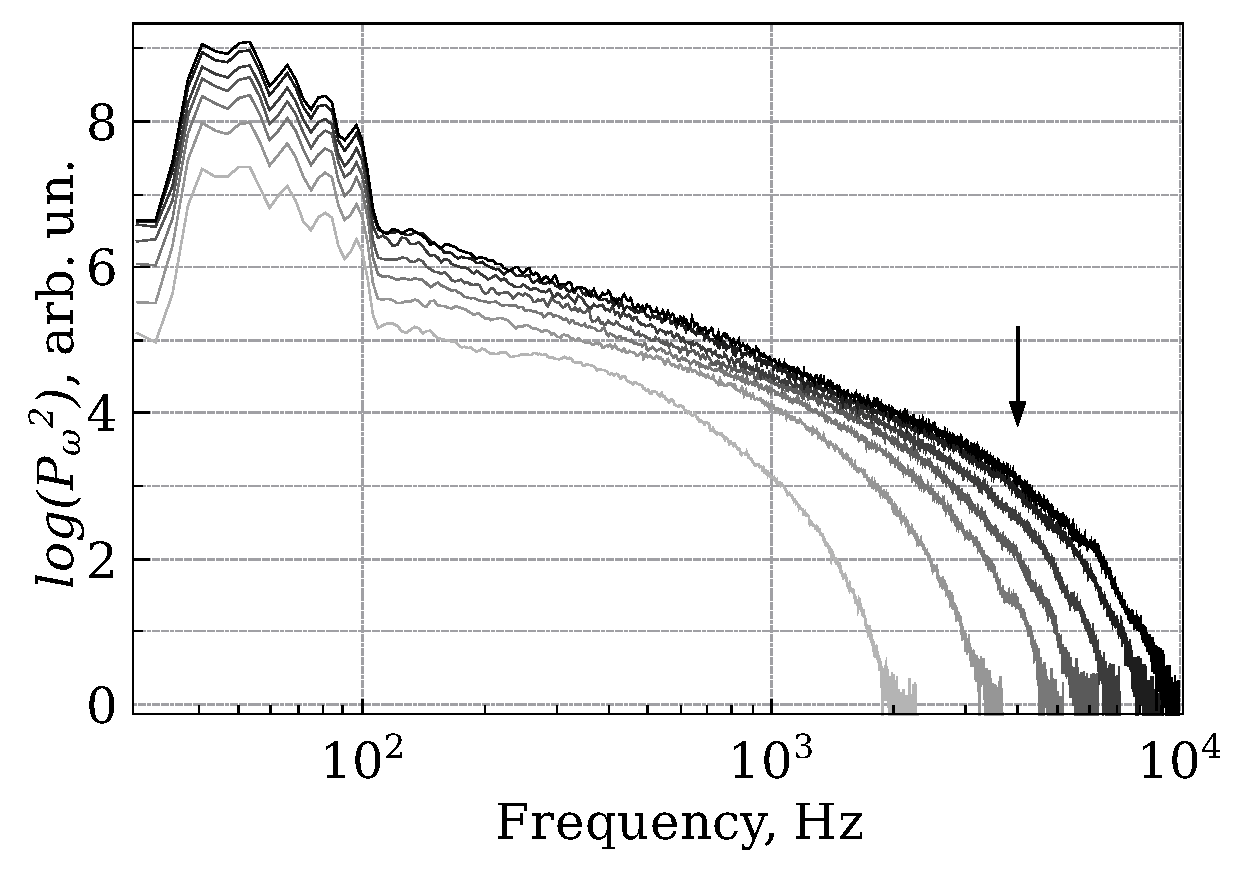
\includegraphics [scale=.8] {article1/spectra_dlog.eps}
  \caption{Спектры поверхностных колебаний $P^2_\omega$ возбужденных случайной силой в частотном диапазоне 39-103 Гц на разных амплитудах возбуждающей силы. Среднеквадратичное значение возбуждающего напряжения $V_P$ меняется от 4 до 30 В. Более темные линии соответствуют большей силе накачки. Стрелкой показана высокочастотная граница инерционного интервала $\omega_b \approx 4$ кГц при накачке 30 В.} 
  \label{img:hydr_specrta_dlog}  
\end{figure}

	Турбулентные спектры перестроенные в линейном масштабе на рис. \ref{img:hydr_specrta_log} показывают, что убывание амплитуд волн с частотой после высокочастотной границы инерционного интервала может быть достаточно хорошо описано экспоненциальным затуханием $P_\omega^2 \sim	e^{-\omega/\omega_d}$ в некотором интервале. Подгонка согласуется с начальным предположения, что $\omega \gg \omega_d$, полученный параметр $\omega_d$ значительно меньше, чем частоты из интервала подгонки. Например спектр при напряжении накачки $V_p = 26$ В подгонялся в диапазоне 5-9 кГц с $\omega_d \approx 0.6$ кГц. К сожалению узкий интервал подгонки не позволяет установить показатель степени s "квазипланковского" распределения достаточно точно. Полученные значения $\omega_d$ в несколько раз меньше, чем видимая граница между инерционным интервалом и диссипативной области(см. рис. \ref{img:hydr_specrta_dlog}). Это несоответствие можно отнести к определенной степени свободы в определении граничной частоты, которая может быть перенормирована с помощью некоторой константы.

\begin{figure}[ht] 
  \center
  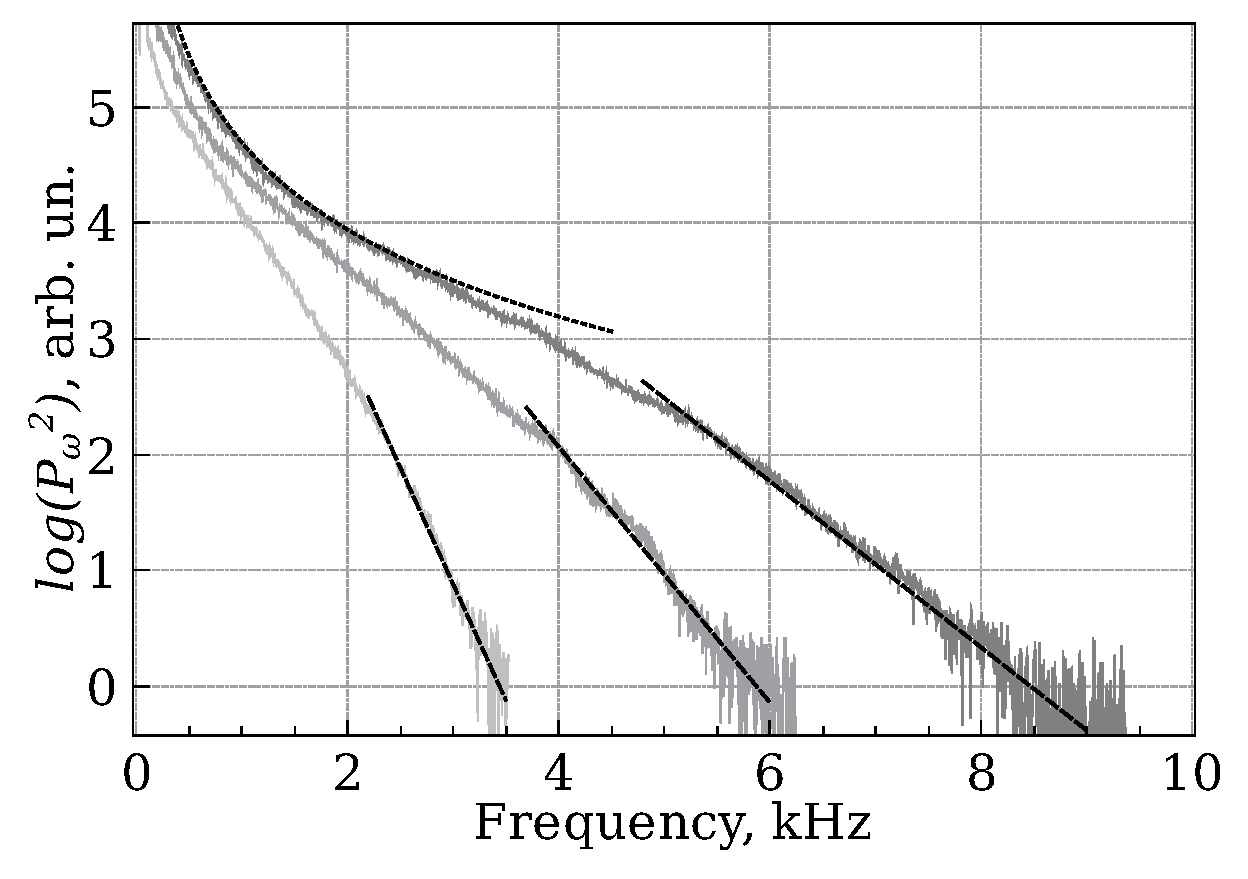
\includegraphics [scale=0.8] {article1/spectra_log.eps}
  \caption{Спектры $P^2_\omega$ для уровней накачки $V_p = 8$ В (светло серая линия), $16$ В (серая линия) и $26$ В (темно-серая линия) в полулогарифмическом масштабе. Линией из точек показан степенной закон $\sim \omega^{-2.8}$, пунктирной линией - подгонка функцией $ \sim e^{-\omega/\omega_d}$. $\omega_d$ примерно равен 0.2, 0.4 и 0.6 для $V_p$ = 8, 16 и 26 В соответственно.} 
  \label{img:hydr_specrta_log}  
\end{figure}

	Частота вязкого затухания диссипативной области  $\omega_d$ наблюденная с помощью подгонки экспоненциального затухания в диссипативной области растет с увеличением возбуждающей силы. Для измерения уровня возбуждения использовался отклик поверхности $\eta_0$, а именно абсолютное значение $P_\omega$ на частоте 53 Гц (положение максимума распределения $P_\omega^2$ внутри области накачки). Величина $\eta_0$ прямо пропорциональна средней высоте волны на той же самой частоте. На рис. \ref{img:hydr_wd} показано, что зависимость граничной частоты от величины возбуждения может быть описана степенным законом $\omega_d(\eta_0) \sim	\eta_0^m$ со значение показателя $m = 0.85 \pm 0.05$. Необходимо заметить, что подгонка экспоненциальных спектров с помощью "квази-Планка" с малым ненулевым $s$ ($|s| \le 2$) слабо влияет на полученный параметр $\omega_d$ (меньше чем на 20\%). Однако эта поправка не изменит показатель степени $m$ в пределах погрешности.

	Наблюдаемый показатель $m \approx 0.85$ значительно отличается от ожидаемого $m = 12/5$ из формулы (3). Стоит отметить, что в случае турбулентных каскадов, возбужденных монохроматической силой, измеренная граничная частота находится в хорошем соответствии с ожиданиями $\omega_d(\eta) \sim \eta^{1.3}$. \todo{ссылка}.
	
\begin{figure}[ht] 
  \center
  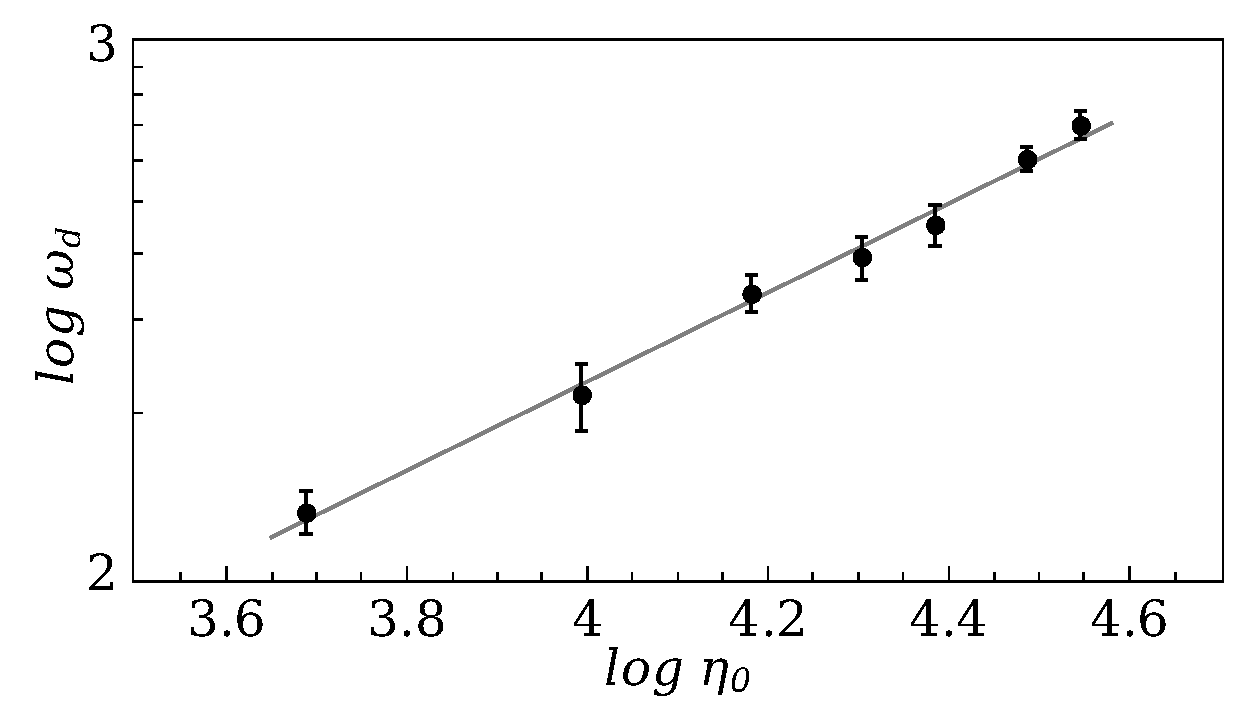
\includegraphics [scale=0.7] {article1/wd.eps}
  \caption{Зависимость частоты вязкого затухания диссипативной области $\omega_d$ (черные точки) от средней высоты низкочастотной волны $\eta_0$, сплошная линия - подгонка функцией $\eta_0^{0.85}$. } 
  \label{img:hydr_wd}  
\end{figure}
\section{Выводы}% \label{sect2_4}

 	Впервые наблюден переход от степенного спектра Колмогова-Захарова в инерционном интервале к “квазипланковскому” распределению $\omega^{-s}e^{-\omega/\omega_d}$ в области диссипации для капиллярной турбулентности. Экспоненциальный спад в области диссипации $\omega/\omega_d \gg 1$ соответствует теоретическому ожиданию и качественно соответствует численным вычислениям \cite{Ryzhenkova1990}. Граница вязкого затухания $\omega_d$ растет с увеличением амплитуды накачки и зависит от средней высоты волны $\eta_0$ на частоте накачки как $\omega_d \sim \eta^{0.85 \pm 0.05}$. Однако наблюденная зависимость отличается от ожидаемой, показатель степени почти в три раза больше, чем предсказанное значение.



\clearpage
